\section{Results and Discussion}
\subsection{Effective Stiffness From Load-Deflection Data}
The effective stiffness was determined to be $13.5 \pm 0.2$ N/m. The effective stiffness was determined by measuring the deflection of the spring under a various known masses under gravitational force. The results of the trial as well as the linear regression forced through the origin can be seen in Figure \ref{fig:Force vs. Deflection}. The plot was forced through the origin since zero force should be observed at zero deflection. The coefficient of determination was found to be $R^2 = 0.9998$, which indicates a strong linear relationship between force and deflection.

From Hooke's, law, the slope of Figure \ref{fig:Force vs. Deflection} is the effective stiffness of the spring, which was found to be $13.5$ N/m. The spring stiffness should be independent of the cart masses as well as the measurement system. 
\begin{figure}[H]
    \centering
    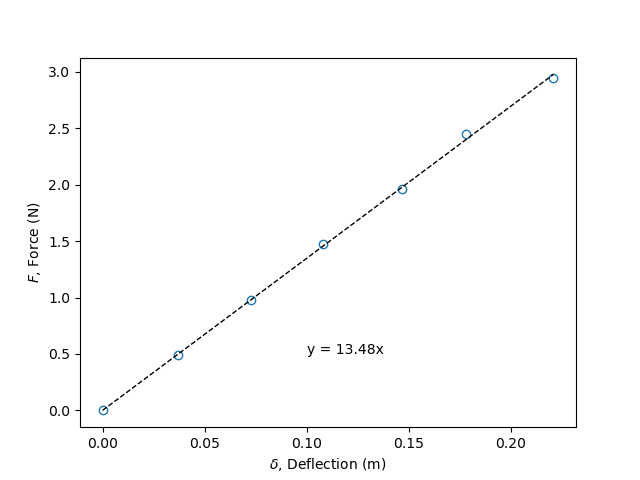
\includegraphics[width=0.5\textwidth]{matplotlib/force vs deflection.png}
    \caption{Force vs. Deflection}
    \label{fig:Force vs. Deflection}
\end{figure}

\subsection{Experimental Resonance}
\begin{table}[H]
    \centering
    \caption{Natural Frequency Data}
    \label{tab:natural_frequency_data_results}
    \begin{tabular}{cccccc}
    \toprule
        & \multicolumn{2}{c}{Small} & \multicolumn{2}{c}{Big} \\
        \cmidrule(lr){2-3} \cmidrule(lr){4-5}
        & $f_{\text{sys}}$ & $f_{\text{no sys}}$ & $f_{\text{sys}}$ & $f_{\text{no sys}}$ \\
        & (Hz) & (Hz) & (Hz) & (Hz) \\
        \midrule
        Derived from period & $1.1317 \pm 0.013$ & $0.9096 \pm 0.009$ & $0.8576 \pm 0.012$ & $0.7513 \pm 0.016$ \\
        Derived from using $k_e$ and $m_e$ & 1.1355 & 0.9221 & 0.8744 & 0.7651 \\
        Relative error (\%) & 0.3286 & 1.3536 & 1.9203 & 1.7989 \\
        \bottomrule
    \end{tabular}
\end{table}
The natural frequencies of the mass-cart with and without measurement system for experimental and theoretical values are shown in Table \ref{tab:natural_frequency_data_results}.The period of 10 cycles was determined experimentally by displacing the mass and measuring the time it took to complete 10 cycles. Details of the analysis can be found in Appendix \ref{app:Natural Frequency Derivation}. The natural frequency of the system was found to be $1.1317 \pm 0.013$ Hz for the small cart with the measurement system, $0.9096 \pm 0.009$ Hz for the small cart without the measurement system, $0.8576 \pm 0.012$ Hz for the big cart with the measurement system, and $0.7513 \pm 0.016$ Hz for the big cart without the measurement system.

The theoretical natural frequencies were calculated using the effective stiffness and effective mass. Effective stiffness was found to be $k_e = 13.5 \pm 0.2$ N/m, and the effective mass was found by using Eq. (\ref{eq:Equivalent Mass Equation of Motion}), as summarized in Table \ref{tab:effective_stiffness_mass_results}. The theoretical natural frequencies were found to be $1.1355$ Hz for the small cart with the measurement system, $0.9221$ Hz for the small cart without the measurement system, $0.8744$ Hz for the big cart with the measurement system, and $0.7651$ Hz for the big cart without the measurement system. 

The experimental natural frequencies were found to be within $0.3286\%$ to $1.9203\%$ of the theoretical values. The theoretical values were slightly higher than the experimental values, which could be due to neglecting the mass of the spring and the mass of the cable. In addition, the experimental period calculations neglected the effects of damping, which would would impact the calculation of the natural frequency.

\subsection{Damping Ratio}
The time response of the amplitude of the small and big carts can be seen in Figures \ref{fig:Big Cart Amplitude vs. Time Trial 1}, \ref{fig:Big Cart Amplitude vs. Time Trial 2}, \ref{fig:Small Cart Amplitude vs. Time Trial 1}, and \ref{fig:Small Cart Amplitude vs. Time Trial 2}. The damping ratio was calculated using the logarithmic decrement method (Eq. \ref{eq:Damping Ratio Calculated With Delta}) and shown in Appendix \ref{app:Damping Ratio Calculation}. The average damping ratio was taken from the linear region (first 6 cycles) as shown in Figures \ref{fig:Big Cart Damping Ratio} and \ref{fig:Small Cart Damping Ratio}. The average damping ratios were found to be $\zeta_{\text{small}, 1, 2} = 0.021, 0.016$ and $\zeta_{\text{big}, 1, 2} = 0.027, 0.023$.  

The discrepancy between the two damping ratios obtained for each trial is due to the non-linear nature of the damping in the system as it approached small amplitudes. The theory suggests, for a linear viscous damping model, that the damping ratio would remain constant, independent of the cycle. From Figures \ref{fig:Big Cart Damping Ratio} and \ref{fig:Small Cart Damping Ratio}, the damping ratio was found to change nearly every cycle, increasing exponential-like. This is not consistent with the linear viscous damping model. The linear viscous damping model does not accurately represent the energy dissipation in the air track system at small amplitudes. 

Further work could be done in displacing the cart by a larger amplitude to see if the damping ratio remains constant initially. Other effects that could be considered are the effects of friction from the air track, torsional friction in the pins of the pulleys, and the mass of the springs and cables.

\begin{figure}[H]
    \centering
    \begin{minipage}{0.45\textwidth}
        \centering
        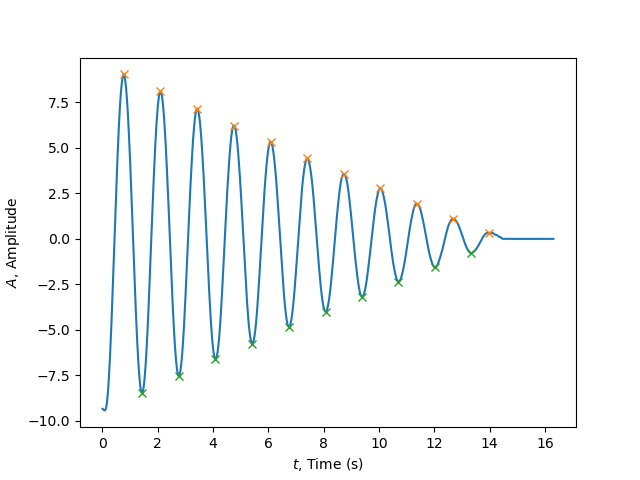
\includegraphics[width=0.9\textwidth]{Sections/Figures/damping_ratio_big_cart_1.png}
        \caption{Big Cart Amplitude vs. Time for Trial 1}
        \label{fig:Big Cart Amplitude vs. Time Trial 1}
    \end{minipage}\qquad
    \begin{minipage}{0.45\textwidth}
        \centering
        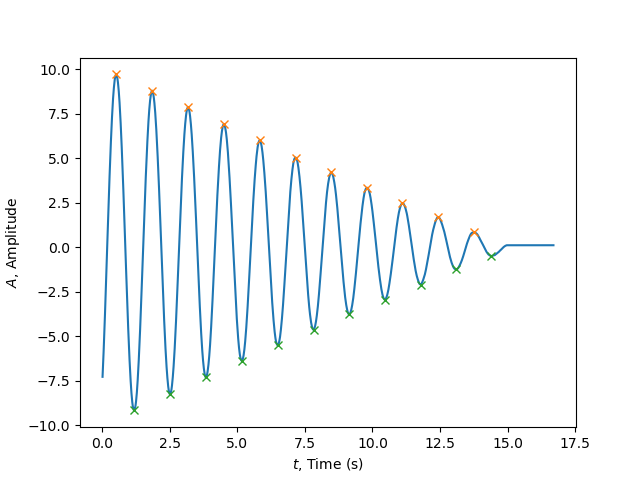
\includegraphics[width=0.9\textwidth]{Sections/Figures/damping_ratio_big_cart_2.png}
        \caption{Big Cart Amplitude vs. Time for Trial 2}
        \label{fig:Big Cart Amplitude vs. Time Trial 2}
    \end{minipage}
\end{figure}
\begin{figure}[H]
    \centering
    \begin{minipage}{0.45\textwidth}
        \centering
        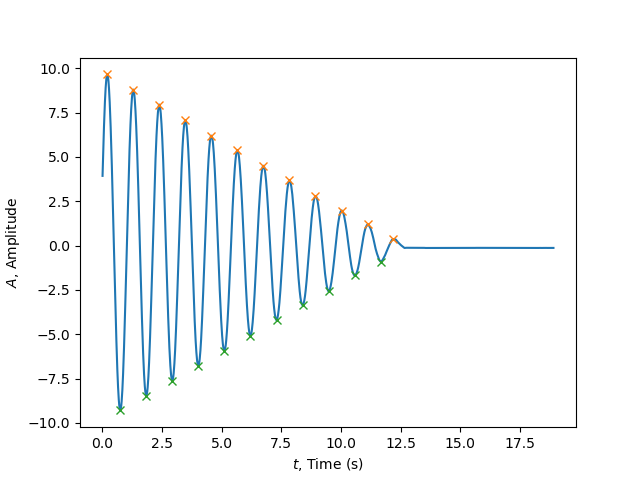
\includegraphics[width=0.9\textwidth]{Sections/Figures/damping_ratio_small_cart_1.png}
        \caption{Small Cart Amplitude vs. Time for Trial 1}
        \label{fig:Small Cart Amplitude vs. Time Trial 1}
    \end{minipage}\qquad
    \begin{minipage}{0.45\textwidth}
        \centering
        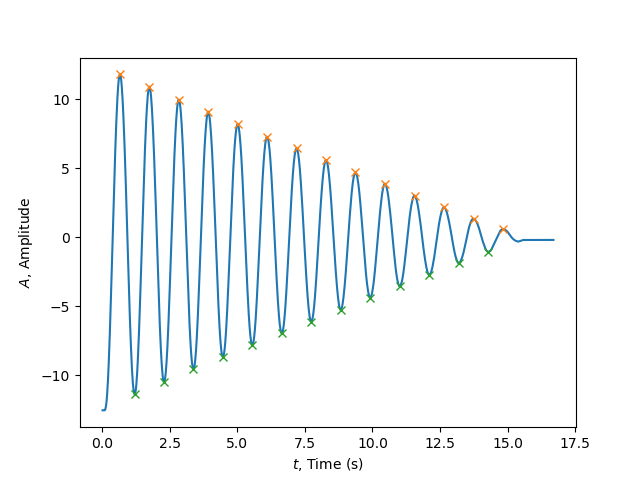
\includegraphics[width=0.9\textwidth]{Sections/Figures/damping_ratio_small_cart_2.png}
        \caption{Small Cart Amplitude vs. Time for Trial 2}
        \label{fig:Small Cart Amplitude vs. Time Trial 2}
    \end{minipage}
\end{figure}
\begin{figure}[H]
    \centering
    \begin{minipage}{0.45\textwidth}
        \centering
        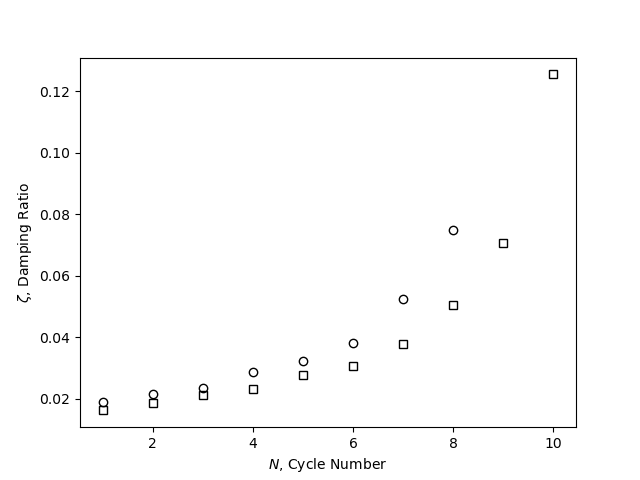
\includegraphics[width=0.9\textwidth]{matplotlib/big cart damping ratio.png}
        \caption{Big Cart Damping Ratio Vs. Cycle Number}
        \label{fig:Big Cart Damping Ratio}
    \end{minipage}\qquad
    \begin{minipage}{0.45\textwidth}
        \centering
        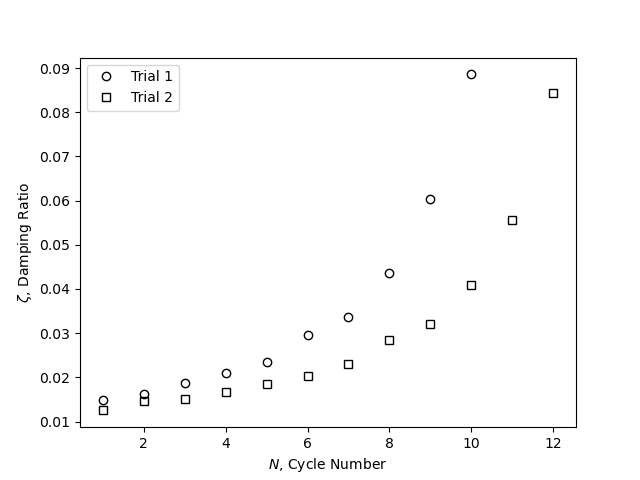
\includegraphics[width=0.9\textwidth]{matplotlib/small cart damping ratio.png}
        \caption{Small Cart Damping Ratio Vs. Cycle Number}
        \label{fig:Small Cart Damping Ratio}
    \end{minipage}
\end{figure}

\subsection{Dynamic Magnification Factor}
The dynamic magnification factor was calculated using the measured displacements for both masses and plotted against the frequency ratio $\omega/p$ as shown in Figures \ref{fig:Big DMF vs. Omega over P} and \ref{fig:Small DMF vs. Omega over P}. This plot was made from the forced response of the system experiment, which tested the response at four forcing frequencies and constant amplitude, $Y_0 = \qty{3.55}{\centi\meter}$.  

The DMF follows the theoretical curve closely, with the in-phase region being very close to the theory. The out-of-phase region was slightly off, with the amplitude being smaller than expected. This could be due to neglecting some inertial terms, such as the mass of the springs and cables as well as the torsional friction in the pins of the pulleys or the friction from the air track. It also can be noted that the DMF is less than one after $\omega / p = \sqrt{2}$, which follows the theory. More details on the analysis can be found in Appendix \ref{app:dmf}.

\begin{figure}[H]
    \centering
    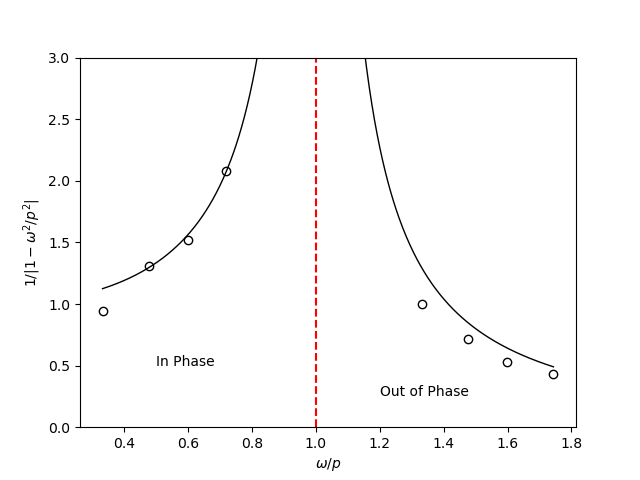
\includegraphics[width=0.5\textwidth]{matplotlib/big dmf vs omega over p.png}
    \caption{Big Cart DMF vs. $\omega/p$}
    \label{fig:Big DMF vs. Omega over P}
\end{figure}
\begin{figure}[H]
    \centering
    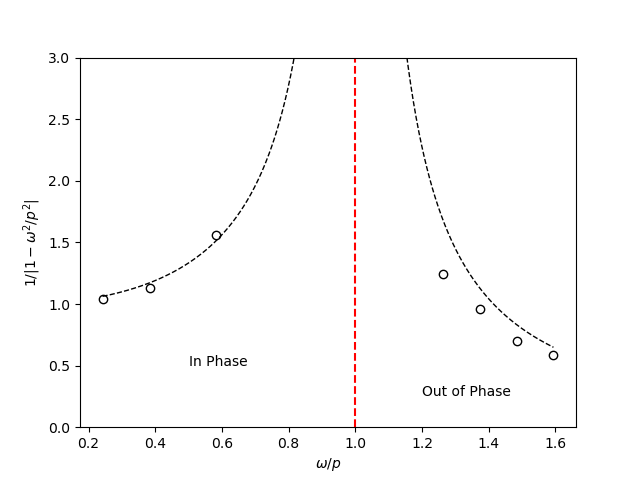
\includegraphics[width=0.5\textwidth]{matplotlib/small dmf vs omega over p.png}
    \caption{Small Cart DMF vs. $\omega/p$}
    \label{fig:Small DMF vs. Omega over P}
\end{figure}

\subsection{Effects of Pulley Measurement System}
The diagram of the pulley system was shown in the theory, Section \ref{sec:Equivalent Mass}. Assuming the pulley is a uniform disk, the effective mass, $m_e$, was found to be $m_e = m_\text{cart} + 0.5 m_\text{pulley 1} + 0.5 m_\text{pulley 2}$. The partial derivation was shown in Section \ref{sec:Equivalent Mass}, with the full derivation shown in Appendix \ref{app:Equivalent Mass Derivation}.

\begin{table}[H]
    \centering
    \caption{Effective Mass Data}
    \label{tab:effective_mass_data}
    \begin{tabular}{ccc}
        \toprule
        & Small & Big \\
        & (kg) & (kg) \\
        \midrule
        Cart & 0.2648 & 0.4465 \\
        Pulley & 0.2599 & 0.0136 \\
        \bottomrule
    \end{tabular}
\end{table}
\begin{table}[H]
    \centering
    \caption{Effective Mass Data}
    \label{tab:effective_stiffness_mass_results}
    \begin{tabular}{ccc}
        \toprule
        & System & No System \\
        & (kg) & (kg) \\
        \midrule
        $m_e$, Small & $0.40155$ & $0.2648$ \\
        $m_e$, Big & $0.58325$ & $0.4465$ \\
        \bottomrule
    \end{tabular}
\end{table}
The pulleys and carts were measured by a mass balance. The masses are shown in Table \ref{tab:effective_mass_data}. The effective mass of the system was found to be $m_e = 0.40155$ kg for the small cart with the measurement system, $0.2648$ kg for the small cart without the measurement system, $0.58325$ kg for the big cart with the measurement system, and $0.4465$ kg for the big cart without the measurement system. 

The effective mass of the system was found to be higher with the measurement system, which is expected since the pulleys add mass to the system. The inertial effects of the pulley system adds 0.1368 kg to the effective mass.

\subsection{Effective Mass Derived From Free Vibration}
From the free vibration data, as shown in Table \ref{tab:natural_frequency_data_results}, the effective mass was derived using the natural frequencies of the system. The effective mass was found to be $0.4099$ kg for the small cart and $0.5818$ kg for the big cart. The theoretical effective mass was found to be $0.4016$ kg for the small cart and $0.5833$ kg for the big cart. The relative error was found to be $2.09\%$ for the small cart and $0.25\%$ for the big cart. The effective mass was found to be within $2.09\%$ of the theoretical value for the small cart and $0.25\%$ for the big cart. The effective mass was found to be higher than the theoretical value, which could be due to neglecting the mass of the springs and cables, and other inertial effects such as the friction from the air track and the torsional friction in the pins of the pulleys.
\begin{table}[H]
    \centering
    \caption{Effective Mass Data}
    \label{tab:effective_mass_data_for_effective_mass_results}
    \begin{tabular}{ccc}
    \toprule
        & Small Cart & Big Cart \\
        & (kg) & (kg) \\
        \midrule
        Effective Mass from Trials & $0.4099 \pm 0.009$ & $0.5818 \pm 0.020$ \\
        Effective Mass from Theory & 0.4016 & 0.5833 \\
        \midrule 
        Relative Error & 2.09\% & 0.25\% \\
        \bottomrule
    \end{tabular}
\end{table}